\section{Кластеризация}

В общих чертах, цель кластеризации --- найти различные группы внутри элементов данных. Для этого алгоритмы кластеризации находят такую структуру данных, чтобы элементы одного и того же кластера (или группы) были более похожи друг на друга, чем на элементы из разных кластеров. Для примера можно представить, что имеется набор данных фильмов и мы хотим их классифицировать. Имеются следующие обзоры фильмов:

\begin{center}
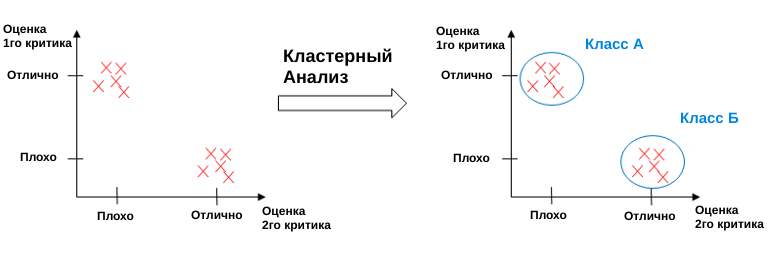
\includegraphics[scale=0.5]{pics/clustering.png}
\end{center}

Модель машинного обучения сможет сделать вывод о существовании двух разных классов, ничего не зная о природе данных.

Эти алгоритмы неконтролируемого обучения имеют невероятно широкий спектр приложений и весьма полезны для решения реальных проблем, таких как обнаружение аномалий, рекомендации систем, группировка документов или поиск клиентов с общими интересами на основе их покупок.

В данной работе мы группируем похожие по смыслу слова с помощью векторного представления слов, полученных с помощью \textit{Word2Vec} \cite{bib5}. 

\textit{Word2Vec} принимает большой текстовый корпус в качестве входных данных и сопоставляет каждому слову вектор, выдавая координаты слов на выходе. Сначала он генерирует словарь корпуса, а затем вычисляет векторное представление слов, «обучаясь» на входных текстах. Векторное представление основывается на контекстной близости: слова, встречающиеся в тексте рядом с одинаковыми словами (а следовательно, имеющие схожий смысл), будут иметь близкие (по косинусному расстоянию) векторы. Полученные векторные представления слов могут быть использованы для обработки естественного языка и машинного обучения.